\documentclass[11pt]{article}
\usepackage[utf8]{inputenc}
\usepackage[margin=2cm]{geometry}
\usepackage{placeins}
\usepackage{graphicx}
\usepackage{wrapfig}
\usepackage{fancyhdr}
\usepackage[svgnames]{xcolor}
\usepackage{listings}
\usepackage{caption}
\usepackage{mwe}
\usepackage{amsmath}
\usepackage[super]{nth}
\usepackage{stackengine}
\usepackage{url}
\def\UrlBreaks{\do\/\do-}
\usepackage{breakurl}
\usepackage[breaklinks]{hyperref}

\hypersetup{urlbordercolor=0 0 0,pdfborderstyle={/S/U/W 1}}
\newcommand\barbelow[1]{\stackunder[1.2pt]{$#1$}{\rule{.8ex}{.075ex}}}

\allowdisplaybreaks

\setlength{\parindent}{0em}

\lstset{language=R,
    basicstyle=\small\ttfamily,
    stringstyle=\color{DarkGreen},
    morekeywords={TRUE,FALSE},
    deletekeywords={data,frame,length,as,character},
    keywordstyle=\color{blue},
    commentstyle=\color{DarkGreen},
}

\pagestyle{fancy}
\fancyhf{}
\rhead{Jonathan Lee (H00255553)}
\lhead{F21SA Coursework Report}
\rfoot{Page \thepage}

\title{\textbf{F21SA Coursework Report}}

\author{By: Lee, Jonathan}
\date{H00255553}

\begin{document}

% \maketitle
\newpage

\section{Introduction}
This report records the analysis, and the predictions made on the wind speeds at the top of Arthur's Seat, based on the given historic wind speeds data. The following is assumed throughout the report.\\
\par Let $X_{1},...,X_{n}$, where $n=1000$, be Independent Identically Distributed (i.i.d) random variables from a $Rayleigh(\sigma)$ distribution, where $\sigma>0$ is an unknown parameter, and probability density function given by
\begin{equation}
    f(x,\sigma) =
    \begin{cases}
        \frac{x}{\sigma^{2}}\mathrm{exp}\left(\frac{-x^{2}}{2\sigma^{2}}\right), & \quad x\geq0\\
        0,  & \quad x<0
    \end{cases}
\end{equation}
\section{Understanding the data}
\begin{minipage}{0.5\textwidth}
    \centering
    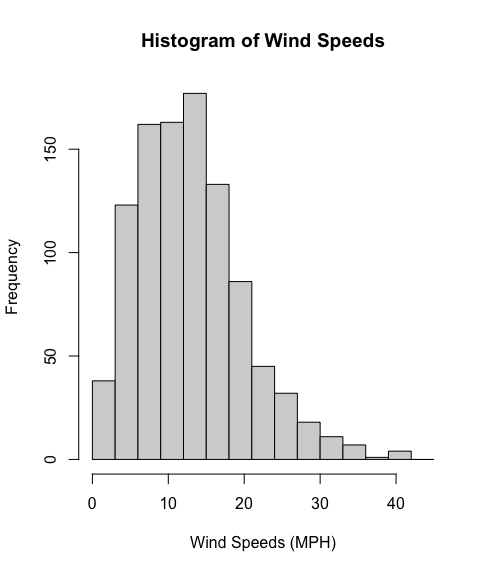
\includegraphics[width = 5cm]{Histogram.png}
    \captionof{figure}{Histogram of Wind Data}
    \label{fig:hist}
\end{minipage}%
\begin{minipage}{0.4\textwidth}
    \centering
    \begin{lstlisting}[caption={Summary Statistics \& S.d of Wind Data},
                        label={list:summary},
                        captionpos=b]
    > summary(wind_data)
           x         
     Min.   : 0.130  
     1st Qu.: 7.615  
     Median :12.145  
     Mean   :12.945  
     3rd Qu.:16.960  
     Max.   :41.870
    > 
    > sd_ori <- sd(wind_data$x); sd_ori
    [1] 6.997126
    >
    > IQR(wind_data$x)
    [1] 9.345
    >
    \end{lstlisting}
\end{minipage}
\par Figure \ref{fig:hist} and listing \ref{list:summary} shows the histogram, and numerical summaries (summary statistics,  standard deviation, and Interquartile range (IQR)) of the set of wind speeds on the top of Arthur's seat. The wind speed data has a mean of $12.945$mph, median of $12.145$mph, standard deviation of $6.997126$mph, Q1 of $7.615$mph, Q3 of $16.960$mph, and an IQR of $9.345$mph. This means, the average wind speed on Arthur's Seat is about $12$ to $13$, and usually not over $16.9$mph or under $7.6$mph, the rest of the numbers are only in the rare cases.\\
\par From the histogram, it could be seen that the distribution is right-skewed, as expected since the wind speeds are modeled after the $Rayleigh(\sigma)$ distribution. This is also perfectly normal since wind speeds cannot be negative, hence a lower bound of $0$mph, and it is possible to record wind speeds of greater than $16.960$mph (\nth{3} quartile), only in some cases. 

\section{Maximum Likelihood Estimator (MLE) for $\sigma$}
The likelihood function is
\begin{equation}
    \begin{split}
        L(\sigma) &= \prod_{n=1}^{n}f(x_{n},\sigma) = \prod_{n=1}^{n}\left[\frac{x}{\sigma^{2}}\exp\left(\frac{-x^{2}}{2\sigma^{2}}\right)\right]
    \end{split}
\end{equation}
The log-likelihood function is
\begin{equation}
    \ell(\sigma) = \log[L(\sigma)] = \left[\sum_{1}^{n}\log(x_{i})\right] -2n\log(\sigma) - \frac{1}{\sigma^{2}}\sum_{1}^{n}\left[\frac{x_{i}^{2}}{2}\right]
\end{equation}
To obtain the MLE for $\sigma$, $\hat{\sigma}$, calculate the root of the first derivative of $\ell(\sigma)$, and solve for 0.
\begin{equation}
    \begin{split}
        \frac{d}{d\sigma}\ell(\sigma) = -2n\left(\frac{1}{\sigma}\right)+2\left(\frac{1}{\sigma^{3}}\right)\sum_{1}^{n}\left[\frac{x_{i}^{2}}{2}\right] = 0
    \end{split}
\end{equation}
\begin{equation}
    % \Longrightarrow \hat{\sigma}_{\mathrm{MLE}} =
    \Longrightarrow \hat{\sigma} =
    \left(\frac{1}{n}\sum_{1}^{n}\left[\frac{x_{i}^{2}}{2}\right]\right)^{\frac{1}{2}}
    = \left(\frac{1}{2n}\sum_{1}^{n}x_{i}^{2}\right)^{\frac{1}{2}}
    \label{eq:mle}
\end{equation}
\section{Fisher's Information $I(\sigma)$ for $\sigma$}
\begin{equation}
    \begin{split}
        nI(\sigma) = -E\left[\frac{d^{2}\ell}{d\sigma^{2}}\right] &= -E\left[\frac{d}{d\sigma}\left(-2n\left(\frac{1}{\sigma}\right)+2\left(\frac{1}{\sigma^{3}}\right)\sum_{1}^{n}\left[\frac{x_{i}^{2}}{2}\right]\right)\right]\\
        &= -E\left[\frac{2n}{\sigma^{2}}-\frac{6}{\sigma^{4}}\left(\frac{1}{2}\right)n(2\sigma^{2})\right]\\
        &=\frac{4n}{\sigma^{2}}, \quad \Longrightarrow I(\sigma) = \frac{4}{\sigma^{2}}
    \end{split}
    \label{eq:fishers}
\end{equation}
Using $Var(\hat{\sigma}) = \frac{1}{I(\sigma)}$, it is deduced that $Var(\hat{\sigma}) \approx \frac{\sigma^{2}}{4}$. That said, $\hat{\sigma}\sim Exp(\frac{2}{\sigma})$.

\section{95\% Confidence Interval (CI) for $\hat{\sigma}$}
Using equations \ref{eq:mle} and \ref{eq:fishers}, a 95\% confidence interval for $\hat{\sigma}$ is
\begin{equation}
    \begin{split}
        \left[\sigma_{L}(\barbelow{x}),\sigma_{U}(\barbelow{x})\right] &= \hat{\sigma} \pm \left(Z_{\frac{\alpha}{2}}\times ese(\hat{\sigma})\right)\\
        &= \hat{\sigma}\pm\left(1.96\times \sqrt{(Var\left(\hat{\sigma}\right)}\right)
    \end{split}
\end{equation}
Through Simulations in R, $\hat{\sigma}=10.40396$, and $\sqrt{Var\left(\hat{\sigma}\right)}=5.201978$ were calculated, hence, the $95\% \text{ CI for }\hat{\sigma}$, $I=\left[\sigma_{L}(\barbelow{x}),\sigma_{U}(\barbelow{x})\right]=[0.2082665, 20.5996459]$.

\section{Calculating \& Estimating $Y'$}
This section aims to Calculate, Predict and Estimate $Y'$, the mean wind speeds for the next 1000 days.
\subsection{Simulation of $Y'$}
\par By letting $X'_{i}\sim\text{Rayleigh}(\hat{\sigma})$, and $Y' = \frac{1}{1000}\sum_{i=1}^{1000}X'_{i}$ be the predicted mean wind speeds for the next 1000 days, R was used to simulate the predicted wind speeds and estimate the distribution of $Y'$. The number of times of simulation was set at 10,000 times, and by using the \verb|rrayleigh(n, scale = 1)| function from the \verb|VGAM| package | where n is the number of observations, and scale being the $\text{Rayleigh}(\hat{\sigma})$ parameter |, the histogram and numerical summaries of the observation is shown in figure \ref{fig:histy} and listing \ref{list:summaryy}.\\
\par Following the results, it could seen that within the next three years, the average mean speed for this period would stay in the range of $12.18$mph and $13.85$mph, with an interquartile range of $0.2902123$mph. Even the mean value of the simulated results, $13.04$mph is not far off from the mean value of the current three years $12.945$mph.

\begin{minipage}{0.4\textwidth}
    \centering
    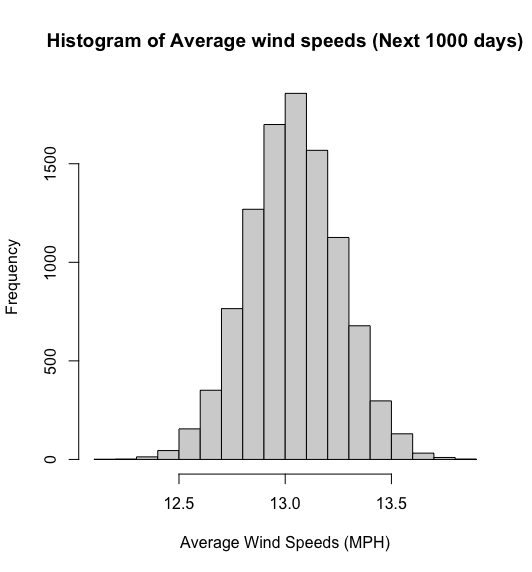
\includegraphics[width = 5.5cm, height = 6.3cm]{YHist.png}
    \captionof{figure}{Histogram of $Y'$}
    \label{fig:histy}
\end{minipage}%
\begin{minipage}{0.6\textwidth}
    \centering
    \begin{lstlisting}[caption={Summary Statistics of $Y'$},
                        label={list:summaryy},
                        captionpos=b]
    > summary(Y)
     Min.  1st Qu. Median  Mean   3rd Qu. Max. 
    12.18  12.89   13.04   13.04  13.18   13.85 
    >
    > sd(Y)
    [1] 0.2154952
    >
    > IQR(Y)
    [1] 0.2902123
    >
    > quantile(Y, c(0.025, 0.975))
        2.5%    97.5% 
    12.61386 13.46574
    >
    >
    \end{lstlisting}
\end{minipage}\\

\subsection{Larger Range of wind speeds in the Coming Three Years?}
Researchers believe that the the variance of wind speeds will increase over the years, where $P[\text{sd}(Z')>\text{sd}(\barbelow{x})]$, $\text{sd}(Z')$ is the standard deviation of the predicted sample of future wind speeds, $Z' = (X'_{1},...,X'_{1000})$, and $\text{sd}(\barbelow{x})$ is the standard deviation of speeds in the current three years. \\
\par Given $P[\text{sd}(Z')>\text{sd}(\barbelow{x})] =P[\text{sd}(X'_{1},...,X'_{1000})>\text{sd}(\barbelow{x})]$, and let variable $k=0$, for each event $\{\text{sd}(X'_{i})>\text{sd}(\barbelow{x})\},\text{ where }i = 1,2,...,1000$ that is true, we add $1$ to the variable $k$. At the end of the simulation, to obtain the value of $P[\text{sd}(Z')>\text{sd}(\barbelow{x})]$, we simply take $\frac{k}{\text{number of simulations}}$.\\
\par Through simulations in R, we obtain a value where $P[\text{sd}(Z')>\text{sd}(\barbelow{x})]=0.1342$, and $\frac{1342}{10000}$ simulations return a standard deviation that is greater than the standard deviation of the current three years.

\subsection{Using the CI's of $\barbelow{x}$, $I$, to check its Robustness}
\begin{figure}[!ht]
    \centering
    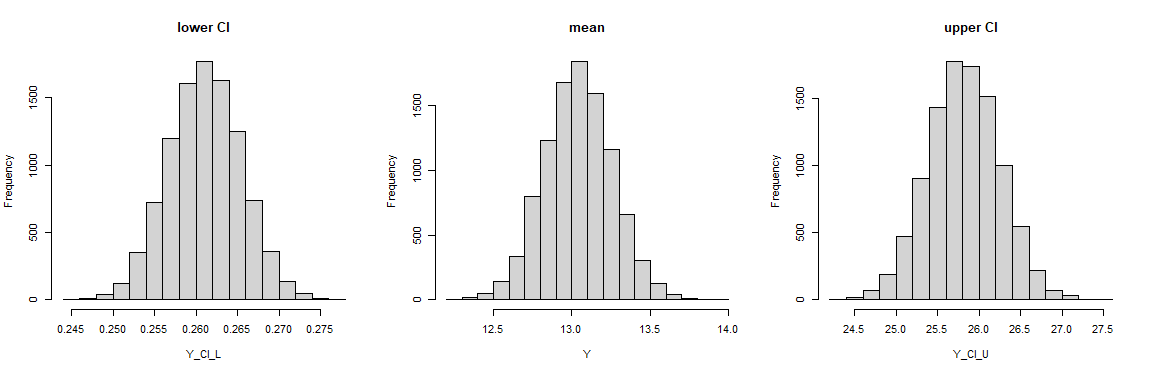
\includegraphics[width=\textwidth]{closeup.png}
    \caption{Individual Histograms of Mean and CI's of $\text{sd}(Z)$}
    \label{fig:closeup}
\end{figure}
\begin{figure}[!ht]
    \centering
    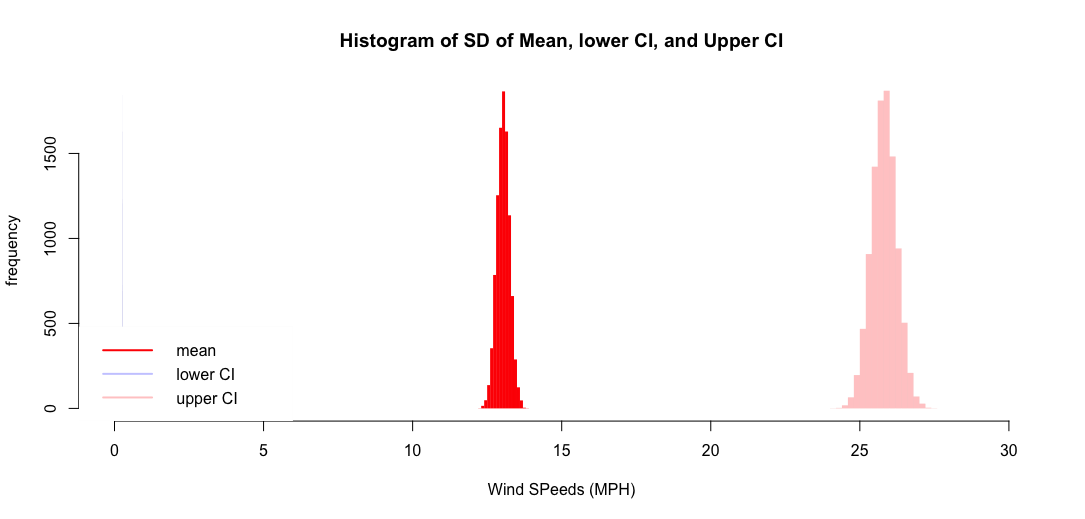
\includegraphics[width=13cm]{567Hist.png}
    \caption{Histograms of Mean and CI's of $\text{sd}(Z)$}
    \label{fig:spread}
\end{figure}
\FloatBarrier
Figure \ref{fig:closeup} and \ref{fig:spread} shows the histograms of CI's and Means of $Z$. Let $X^{'}_{i_{LowCI}}\sim\text{Rayleigh}(\sigma_{L}(\barbelow{x}))$, and $X^{'}_{i_{UpperCI}}\sim\text{Rayleigh}(\sigma_{U}(\barbelow{x}))$.\\
\par to check for robustness of $Z$, $P[\text{sd}(Z^{'}_{LowCI})>
\text{sd}(\barbelow{x})]$, and $P[\text{sd}(Z^{'}_{UpperCI})>
\text{sd}(\barbelow{x})]$ were calculated, where $Z^{'}_{LowCI}$ and $Z^{'}_{UpperCI}$ were predicted means of $\left[\sigma_{L}(\barbelow{x}),\sigma_{U}(\barbelow{x})\right]=[0.2082665, 20.5996459]$. Retrospectively, $Z^{'}_{LowCI}\sim\text{Rayleigh}(\hat{\sigma}_{LowCi})$, and $Z^{'}_{UpperCI}\sim\text{Rayleigh}(\hat{\sigma}_{UpperCi})$.\\
\par From the results from simulation in R, over 10000 iterations, results show $P[\text{sd}(Z^{'}_{LowCI})>
\text{sd}(\barbelow{x})]=0$, and $P[\text{sd}(Z^{'}_{UpperCI})>
\text{sd}(\barbelow{x})]=0.8407$. The explanation for the probabilities are simple. It is due to the positive-skewed, and non-negative nature of the distribution, where, the higher $\hat{\sigma}$ is, the higher the standard deviation yield. And since $\hat{\sigma}_{UpperCi}>\hat{\sigma}_{MLE}>\hat{\sigma}_{LowCI}$, it is only logical that $P[\text{sd}(Z^{'}_{UpperCI})>\text{sd}(\barbelow{x})]>P[\text{sd}(Z')>\text{sd}(\barbelow{x})]>P[\text{sd}(Z^{'}_{LowCI})>
\text{sd}(\barbelow{x})]$. 
\section{Conclusion}
The prediction of wind speeds over the next 1000 days yielded very different results due to the large upper and lower bounds of $\hat{\sigma}$, caused by the large CI range. This means that the model and results are not robust towards the change in $\sigma$, hence the estimation of sigma within the model is very important and a slightest deviation in that will lead to very different results. 

\newpage
\section{Appendices}
% \tableofcontents
% \newpage
\subsection{R-Code}
\textbf{Link to GitHub:} \href{https://github.com/jonleesy/F21SA-Coursework}{\underline{https://github.com/jonleesy/F21SA-Coursework}}
\par Recommend the Viewing of RAW code on GitHub, due to the formatting of \LaTeX.
\lstinputlisting[language=R]{../F21SA_H00255553.R}
\newpage
\begin{thebibliography}{9}

\bibitem{}
\url{DataAnalytics.org.uk} (2019) \textit{Plot two (overlapping) histograms on one chart in R}. Available At: \url{https://www.dataanalytics.org.uk/plot-two-overlapping-histograms-on-one-chart-in-r/} Accessed: 31 Oct 2021

\bibitem{}
MIT Open Course Ware (No Date) \textit{ML and MOM Estimates of Rayleigh Distribution Parameter}. Available At: \url{https://ocw.mit.edu/ans7870/18/18.443/s15/projects/Rproject3_rmd_rayleigh_theory.html} Accessed: 28 Oct 2021

\bibitem{}
Goual. H, Et al., (2019) `Validation of Burr XII inverse Rayleigh model via a modified chi-squared goodness-of-fit test', \textit{Journal of Applied Statistics}, pp. 393-423. doi: 10.1080/02664763.2019.1639642



\end{thebibliography}
\end{document}
